The system used in the case studies here reported has been developed to support identification of features that could be used to project emotions with a non-bio-inspired platform. This system is composed of two complementary parts: robotic platform and emotional enrichment system. The platform has been envisioned to be as simple as possible without any resemblance to anthropomorphic embodiment, while the emotional enrichment has been designed to be applied also to other platforms and to be extended to other emotion expressions.
 
\subsection{Robotic Platform}
The platform is a holonomic base, shown in Figure~\ref{fig:holonomic-platform}. The first prototype included three metal gear motors with encoders, an Arduino Mega micro-controller, one servo motor and X-Bee system to enable the communication between Arduino and a remote computer. The mechanical design of the prototype is shown in Figure~\ref{fig:triskar-prototype}. A PID controller for each wheel was implemented and tuned to guarantee the desired linear and angular velocity.

This prototype was modified after the first case study to improve the expressiveness of the upper part. Two additional servo motors and mechanical structure to support all these motors were added. The two motors attached to beams could be controlled to obtain an asymmetric or opening-closing movement. 
The third motor deforms the upper part of the foam. Figure~\ref{fig:triskar-first-design} shows the placement of the motors. To hide the structure, foam and a light blue cloth covering the foam were used, as it could be seen in Figure~\ref{fig:triskar-cover}. The light blue color was selected to not generate any particular arousal in people~\cite{Naz2012}. 

Although this version showed the possibility to convey emotions, still it was not autonomous enough to host the emotional enrichment system. Therefore, an Odroid-U3 microcomputer was added, communicating with Arduino Mega via ROS-Serial.
Also, it was decided to make some improvements in the upper part. Two reasons motivated these changes. First the upper deformation was not clearly perceived by subjects; second, the beams were damaging the foam. Therefore, a lever was added to the deformation motor, and a piece of rubber was adopted to safely connect the beams with the foam. The final arrangement is shown in Figure~\ref{fig:triskar-second-design}.
 
The final version, with improved computational power (Arduino Due instead of Mega) is shown in Figure~\ref{fig:triskar-third-design}.
\begin{figure}[h]
	\centering
	\begin{subfigure}[c]{0.3\textwidth}
	\centering
	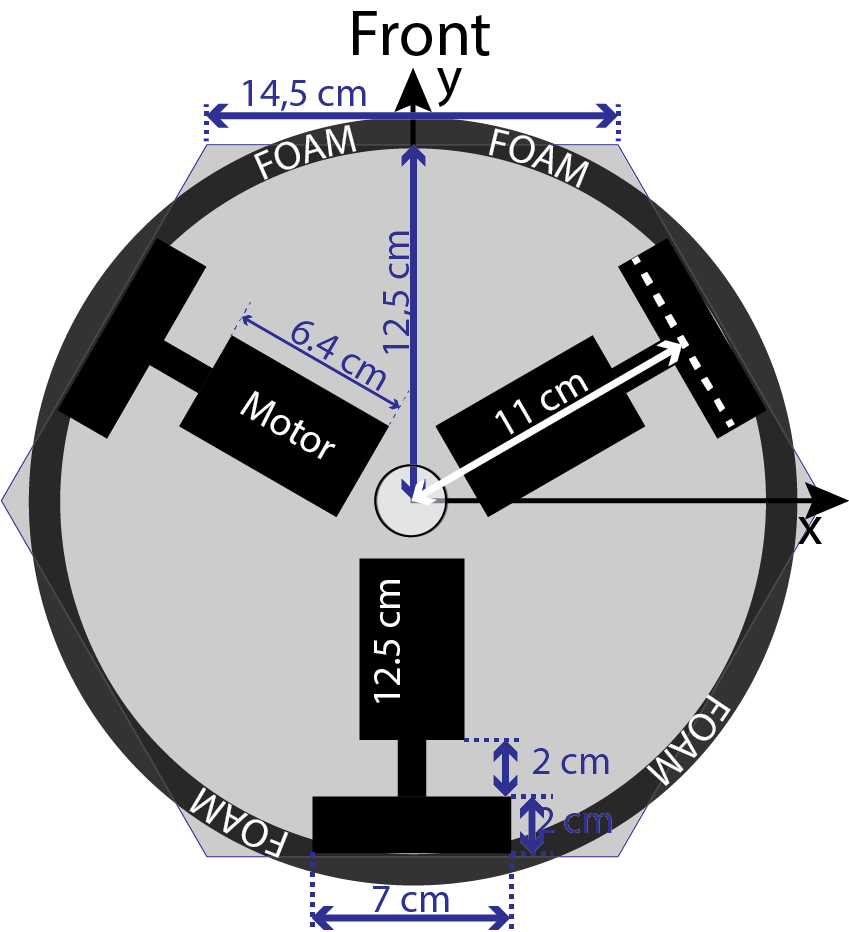
\includegraphics[width=\textwidth]{./Images/TriskarThird.png}
	\caption{Holonomic Base used in all the platform's version.}
	\label{fig:holonomic-platform}
	\end{subfigure}
	\begin{subfigure}[c]{0.3\textwidth}
	\centering
	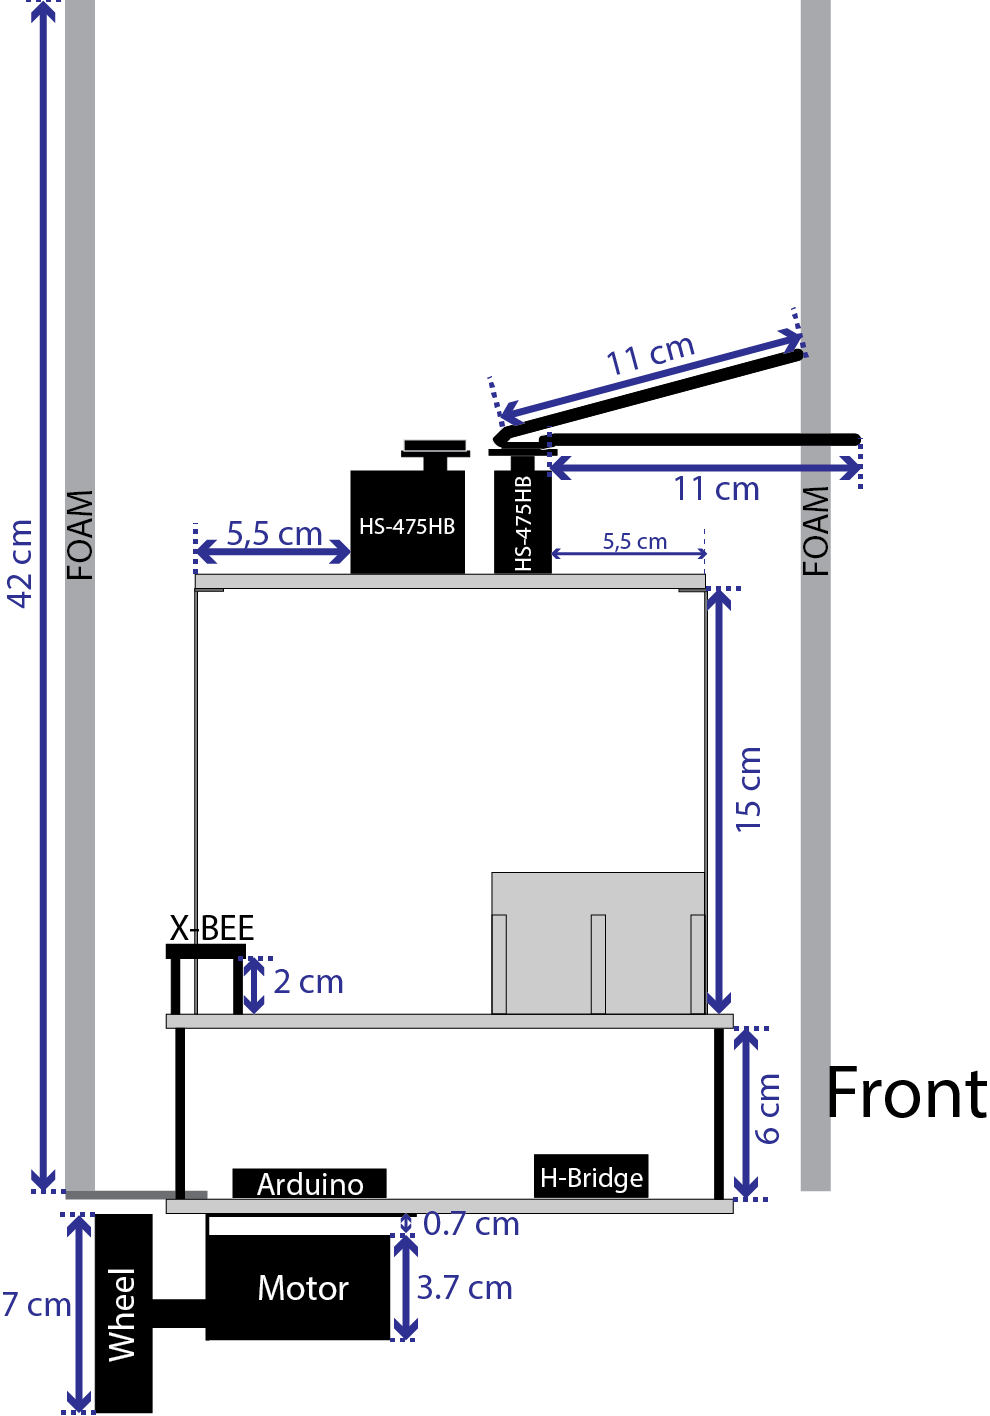
\includegraphics[width=\textwidth]{./Images/upperSecondC.png}
	\caption{First version blueprint.}
	\label{fig:triskar-first-design}
	\end{subfigure}
	\begin{subfigure}[c]{0.3\textwidth}
	\centering
	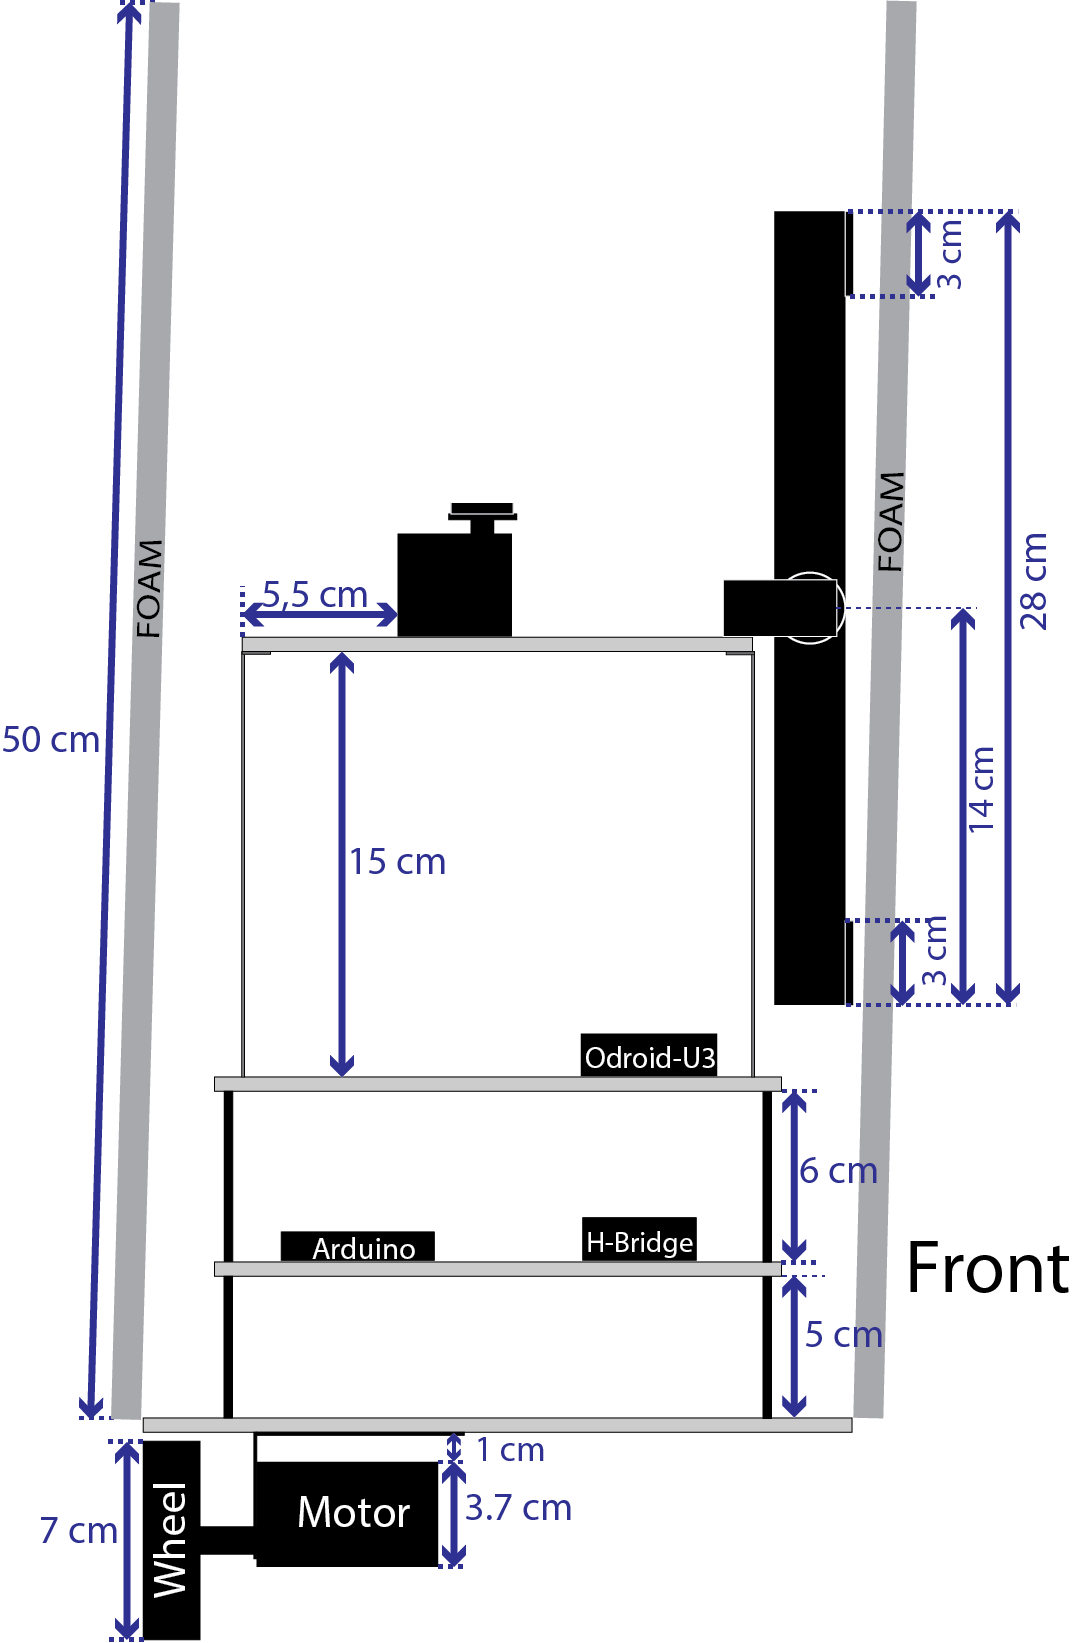
\includegraphics[width=\textwidth]{./Images/upperThirdD.png}
	\caption{Second version blueprint.}
	\label{fig:triskar-second-design}
	\end{subfigure}
	\\
	\begin{subfigure}[c]{0.3\textwidth}
	\centering
	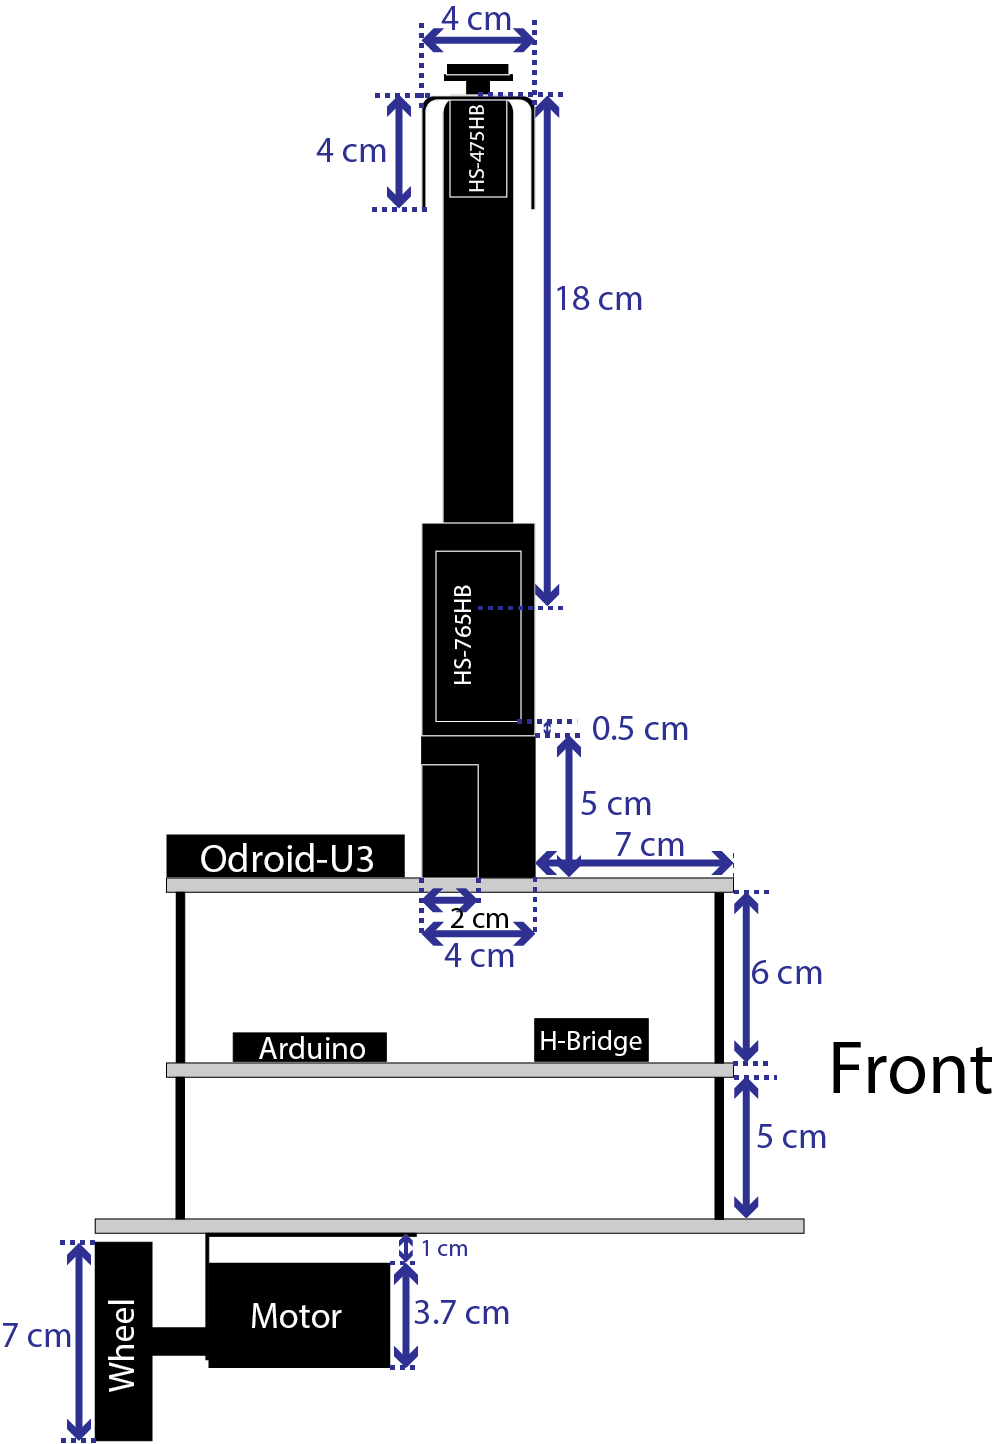
\includegraphics[width=\textwidth]{./Images/upperFourthD.png}
	\caption{Third version blueprint.}
	\label{fig:triskar-third-design}
	\end{subfigure}
	\begin{subfigure}[c]{0.3\textwidth}
	\centering
	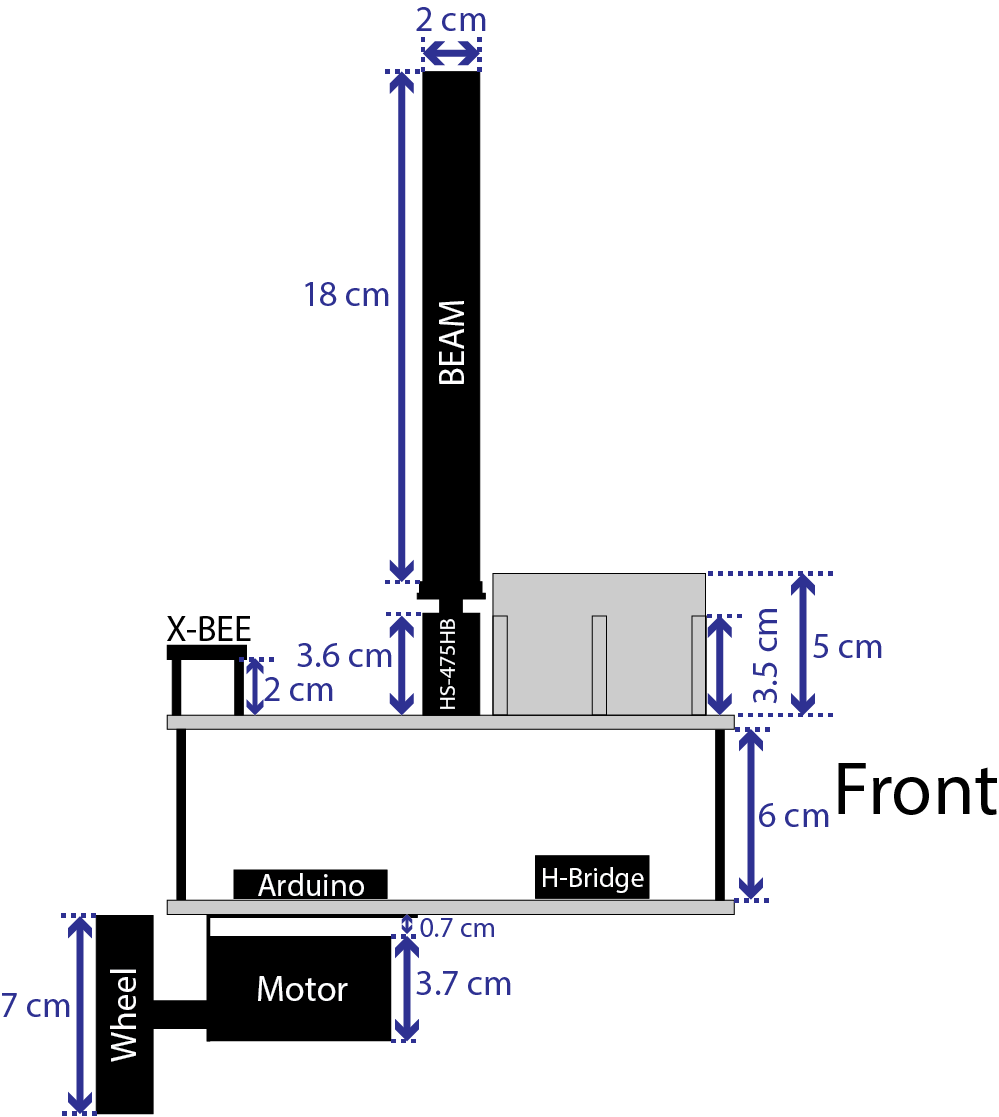
\includegraphics[width=\textwidth]{./Images/upperFirstB.png}
	\caption{Final version blueprint.}
	\label{fig:triskar-prototype}
	\end{subfigure}
	\begin{subfigure}[c]{0.3\textwidth}
	\centering
	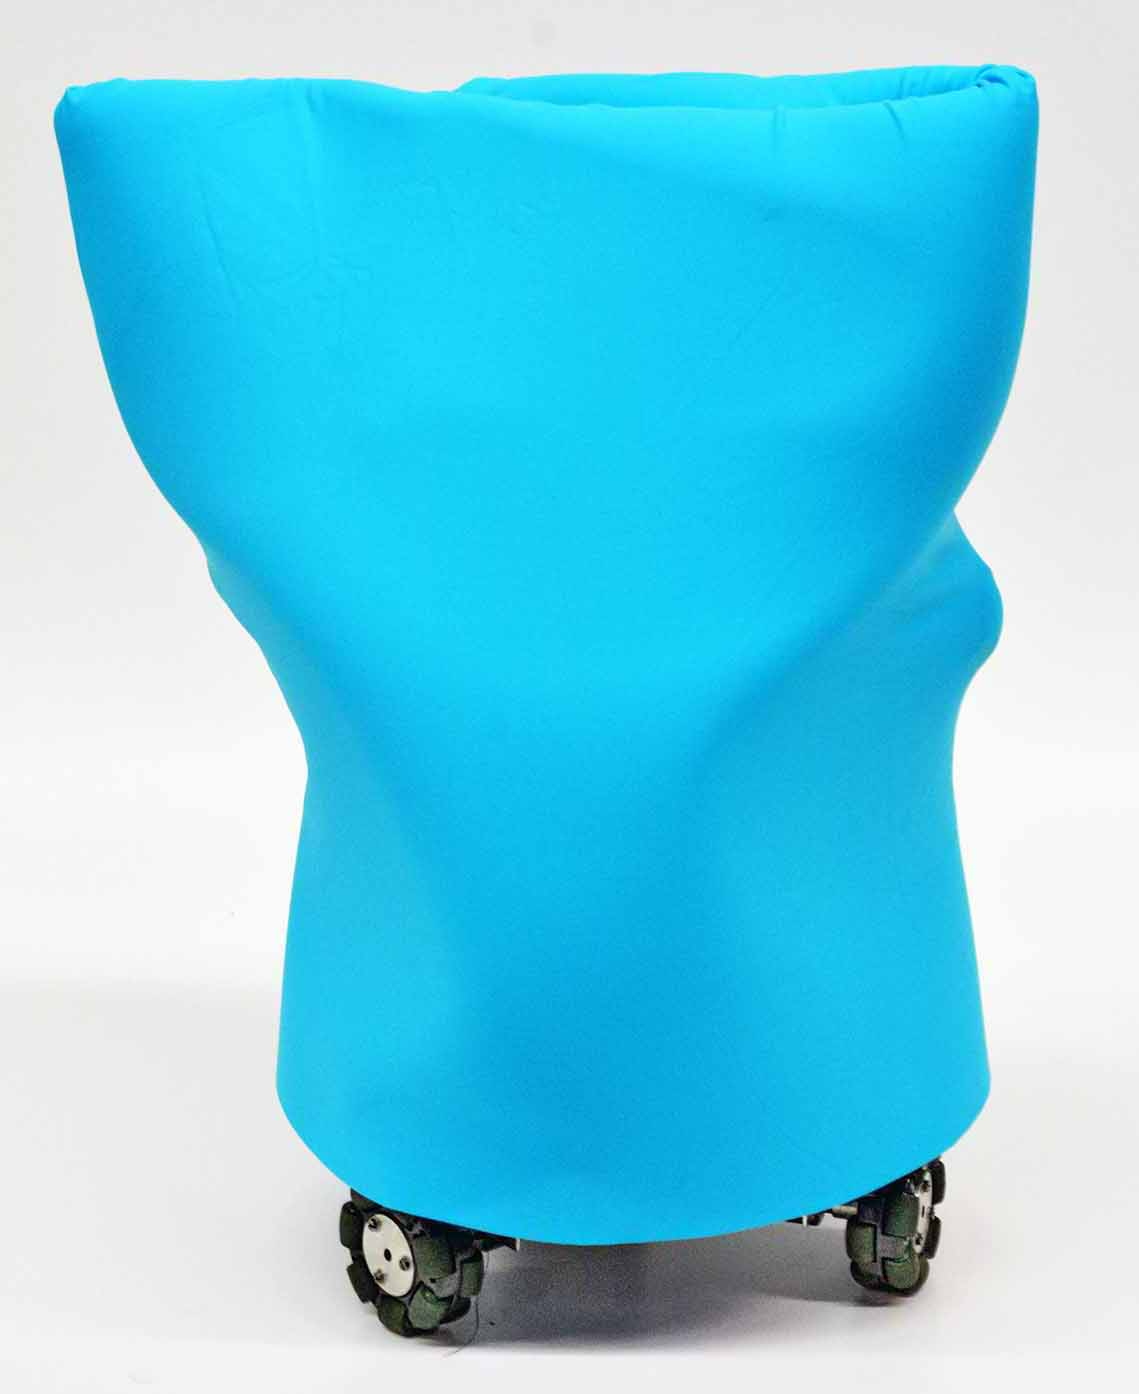
\includegraphics[width=\textwidth]{./Images/Triskar2.jpg}
	\caption{Platform with cover.}
	\label{fig:triskar-cover}
	\end{subfigure}
	\caption{Triskarino platform.}
	\label{fig:robot}
\end{figure} 